    \section*{Exercício 3}
    \addcontentsline{toc}{section}{Exercício 3}
    
    Seja o pólo $s=0$ através da transformação conforme $z = e^{T_s s}$ corresponde ao pólo $z = 1$.
    
        \begin{enumerate}
        
        \item % A
        \label{item:ex3a}
        
         Seja $s = \epsilon + i \delta$, com $\epsilon$ e $\delta$ arbitrários, temos que o processo de mapeamento de pólos e zeros tem como condição necessária que o ganho tanto em $s$ quanto em $z$ sejam iguais. Isto significa 
        
            \begin{equation}
                 \lim\limits_{s \rightarrow (0, 0)} \left \lvert G(s) \right \rvert = \lim\limits_{z \rightarrow (1, 0)} \left \lvert G(z) \right \rvert
            \label{eq:limitcond}
            \end{equation}
        
        Então 
        
            \begin{equation}
                \lim\limits_{(\epsilon, \delta) \rightarrow (0, 0)} \left \lvert \frac{1}{\epsilon + j \delta} \right \rvert = \lim\limits_{(\epsilon, \delta) \rightarrow (0, 0)} \left \lvert \frac{K}{e^{T_s \epsilon + i T_s \delta} - 1} \right \rvert
            \end{equation}
        
        Seja $K$ finito, temos que 
        
            \begin{equation*}
                K = \lim\limits_{(\epsilon, \delta) \rightarrow (0, 0)} \left( \frac{(e^{T_s \delta} \cos{T_s \epsilon}  - 1)^2 + e^{2 T_s \delta} \sin^2 T_s \epsilon}{\epsilon^2 + \delta^2} \right)^{\frac{1}{2}}
            \end{equation*}
        
        Para toda curva $\delta = k \epsilon$, $k \in \mathbb{R}$, temos que 
        
            \begin{equation*}
                K = \lim\limits_{\epsilon \rightarrow 0} \left( \frac{(e^{k T_s \epsilon} \cos{T_s \epsilon}  - 1)^2 + e^{2 k T_s \epsilon} \sin^2 T_s \epsilon}{\epsilon^2(1 + k^2)} \right)^{\frac{1}{2}}
            \end{equation*}
        
        Através de manipulações algébricas, obtemos que
        
            \begin{equation}
                K = \lim\limits_{\epsilon \rightarrow 0} \left[ \left(\frac{e^{k T_s \epsilon} \cos{T_s \epsilon}  - 1}{\epsilon}\right)^2 + \left( \frac{e^{k T_s \epsilon} \sin T_s \sin T_s \epsilon}{\epsilon} \right)^2 \right]^{\frac{1}{2}} \frac{1}{\sqrt{1 + k^2}}
            \label{eq:K}
            \end{equation}
                
        O termo à esquerda na expressão do limite em \eqref{eq:K} é uma indeterminação matemática para $\epsilon \rightarrow 0$. Por meio da regra de L'Hôpital, obtemos 
        
            \begin{equation}
                \lim\limits_{\epsilon \rightarrow 0} \frac{e^{k T_s \epsilon} \cos{T_s \epsilon}  - 1}{\epsilon} = \lim\limits_{\epsilon \rightarrow 0} \left( k T_s e^{k T_s \epsilon} \cos{T_s \epsilon} - e^{k T_s \epsilon} \sin{T_s \epsilon} \right) = k T_s
            \label{eq:esqex3a}
            \end{equation}

        O termo à direita em \eqref{eq:K} possui um limite direto e igual a $T_s$. Desta forma, temos que $K = T_s$. Assim, o equivalente em $z$ é dado por 
        
        \begin{equation*}
        G(z) = \frac{T_s}{z - 1} = \stackrel{N}{=} = \frac{0.1}{z - 1}
        \end{equation*}
        
        Perceba que a função de transferência resultante é estritamente própria. Além disso, esta é nomeadamente o inverso da transformação para trás.
        
        \item % B
        
        Para uma função biprópria, o equivalente em z é da forma
        
            \begin{equation}
            G(z) = K \frac{z+1}{z-1}
            \end{equation}
        
        De mesma forma, a equação deve satisfazer a condição \eqref{eq:limitcond}. Assim
        
            \begin{equation}
                \lim\limits_{(\epsilon, \delta) \rightarrow (0, 0)} \left \lvert \frac{1}{\epsilon + j \delta} \right \rvert = \lim\limits_{(\epsilon, \delta) \rightarrow (0, 0)} K \left \lvert \frac{e^{T_s \epsilon + i T_s \delta} + 1}{e^{T_s \epsilon + i T_s \delta} - 1} \right \rvert
            \end{equation}
            
        Para K finito, 
        
            \begin{equation}
                K = \lim\limits_{(\epsilon, \delta) \rightarrow (0, 0)} \left( \frac{(e^{T_s \delta} \cos T_s \epsilon - 1)^2 +  e^{2 T_s \delta} \sin^2 T_s \epsilon}{((e^{T_s \delta} \cos T_s \epsilon + 1)^2 +  e^{2 T_s \delta} \sin^2 T_s \epsilon) (\epsilon^2 + \delta^2)} \right)^{\frac{1}{2}}
            \end{equation}
        
        Para toda curva $\delta = k \epsilon$, $k \in \mathbb{R}$, temos que 

        \begin{equation}
            \begin{split}
                K &= \lim\limits_{\epsilon \rightarrow 0} \left( \frac{(e^{k T_s \epsilon} \cos T_s \epsilon - 1)^2 +  e^{2 k T_s \epsilon} \sin^2 T_s \epsilon}{((e^{k T_s \epsilon} \cos T_s \epsilon + 1)^2 +  e^{2 k \epsilon} \sin^2 \epsilon) \epsilon^2 (1 + k^2)} \right)^{\frac{1}{2}} \\
                & = \lim\limits_{\epsilon \rightarrow 0} \left( \frac{1}{(e^{k \epsilon} \cos \epsilon + 1)^2 +  e^{2 k \epsilon} \sin^2 \epsilon} \frac{(e^{k \epsilon} \cos \epsilon - 1)^2 +  e^{2 k \epsilon} \sin^2 \epsilon}{\epsilon^2} \right)^{\frac{1}{2}} \frac{1}{\sqrt{k^2 + 1}}
            \end{split}
        \end{equation}
        
        O termo à esquerda no limite tem valor definito e igual a $\frac{1}{2}$, $\forall T_s, k \in \mathbb{R}$. O termo à direita já foi calculada no item anterior e sua dedução está em \eqref{eq:esqex3a}. Desta forma, $K = \frac{T_s}{2}$. A expressão encontrada para o integrador em tempo discreto com uma função biprópria é dada por 
        
            \begin{equation}
                G(z) = \frac{T_s}{2} \frac{z + 1}{z - 1} \stackrel{N}{=} 0.05 \frac{z + 1}{z - 1}
            \end{equation}
        
        A expressão acima corresponde nomeadamente à transformação bilinear ou Tustin.
        
    \begin{figure}[H]
        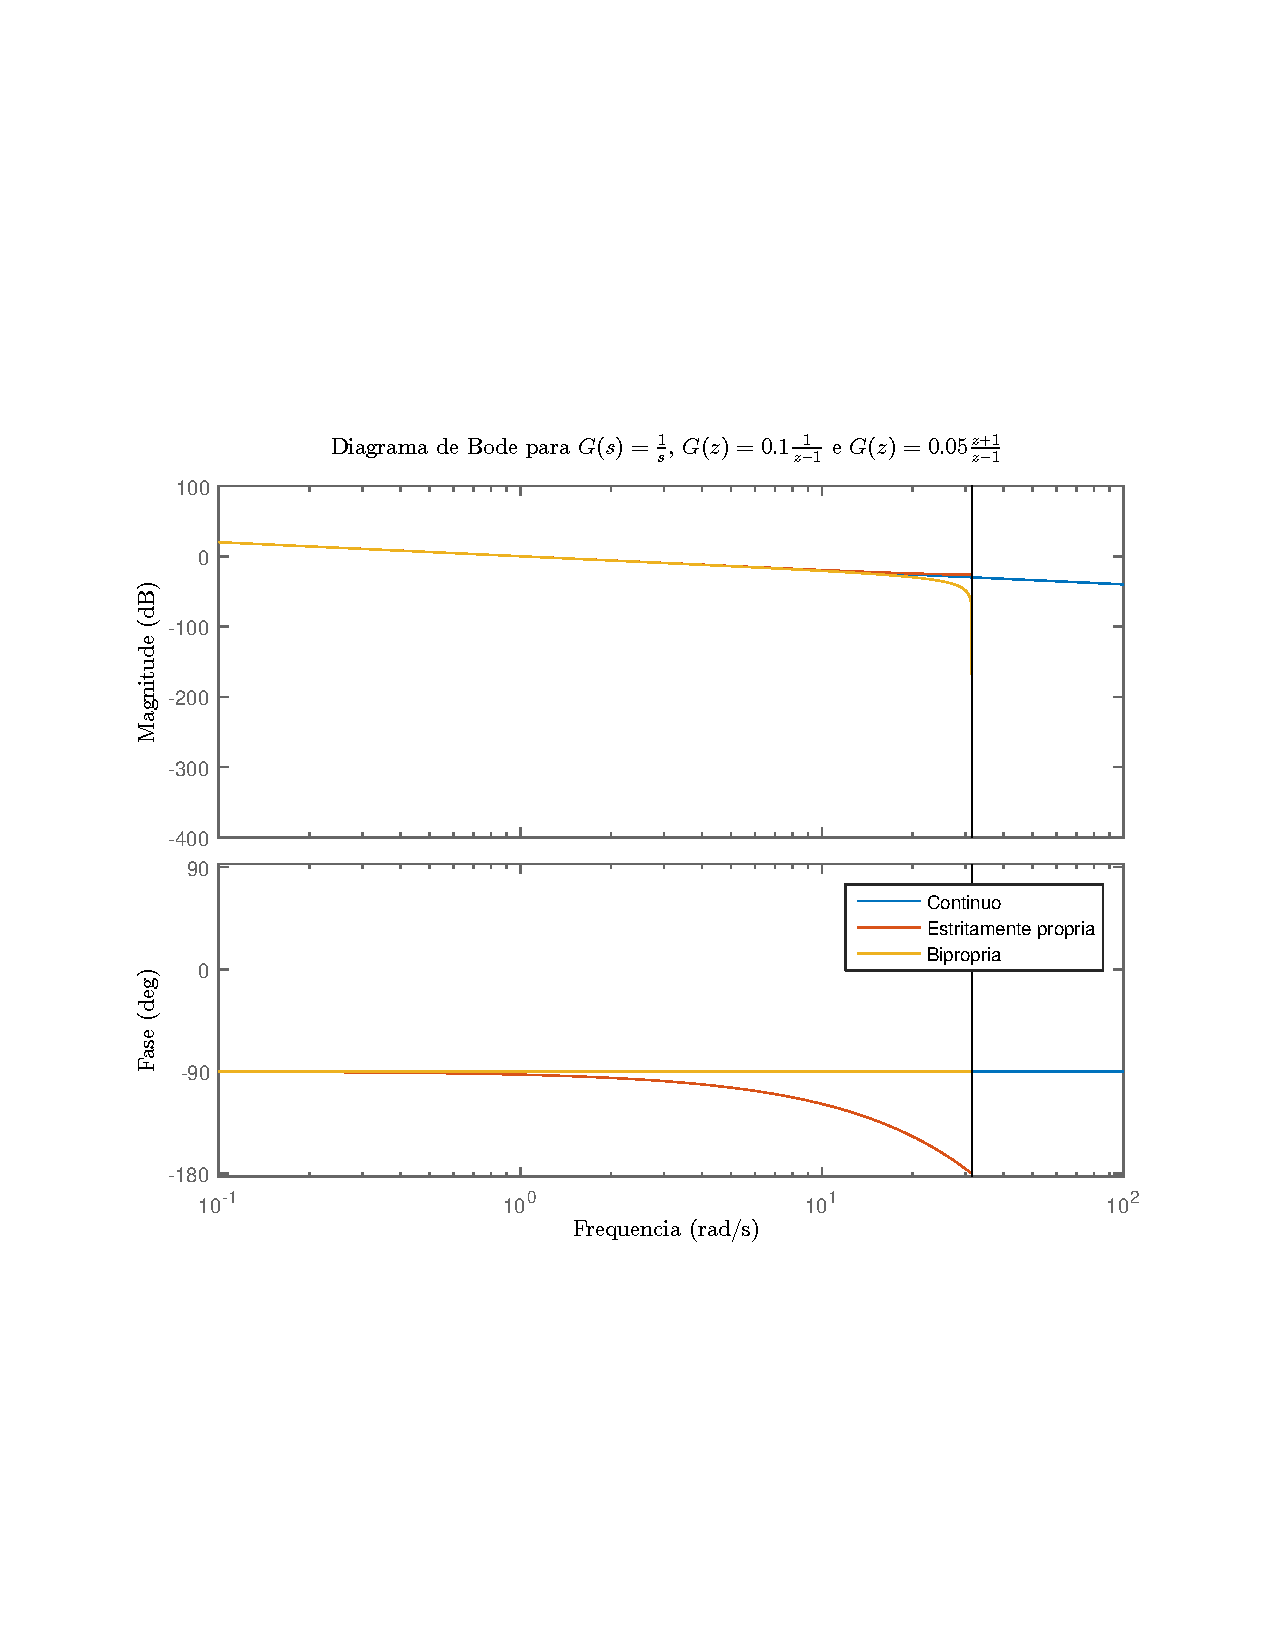
\includegraphics[width=\textwidth]{bodeex3.pdf}
        \caption{\label{fig:ex1ac} Diagrama de bode para as função de transferência contínua, discreta estritamente própria e biprópria} 
    \end{figure}

    \end{enumerate}